\documentclass[10pt,journal,compsoc,onecolumn]{IEEEtran}
\usepackage[utf8]{inputenc}
\usepackage{amsmath,amsfonts,amssymb}
\usepackage{amsthm}
\usepackage{graphicx}
\usepackage{cite}
\usepackage{textcomp}
\usepackage{tikz}
\usetikzlibrary{arrows,positioning,shapes.geometric}
\usepackage{booktabs}
\usepackage{url}

\newtheorem{theorem}{Theorem}
\newtheorem{lemma}[theorem]{Lemma}
\newtheorem{definition}[theorem]{Definition}
\newtheorem{corollary}[theorem]{Corollary}

\begin{document}

\title{A Formal Algorithmic Analysis of Binary Tree Data Structures: Traversal Strategies, View Projections, and Level-Order Processing}

\IEEEtitleabstractindextext{%
\begin{abstract}
Trees represent a fundamental non-linear hierarchical data structure with applications spanning compiler design, database indexing, file system architectures, and network routing. This paper presents a rigorous formal treatment of binary tree structures, establishing definitions for core tree properties including depth, height, and level. We classify binary trees into three canonical forms: Proper (Full), Complete, and Perfect binary trees, and derive bounds on node counts at each level ($2^k$ at level $k$, for a total of $2^{h+1} - 1$ nodes in a perfect tree of height $h$). We formalize the three recursive depth-first traversal strategies --- Pre-order (Root-Left-Right), In-order (Left-Root-Right), and Post-order (Left-Right-Root) --- providing complete implementations and dry-run execution traces. We then introduce the iterative Breadth-First (Level-Order) traversal using a FIFO queue, analyzing its $O(N)$ time and $O(W)$ space complexity where $W$ is the maximum width of the tree. Finally, we formalize Left View and Right View projection algorithms as specialized level-order traversals that extract the first and last visible nodes at each depth level respectively. All algorithms are implemented in Java with formal complexity proofs and illustrative TikZ diagrams.
\end{abstract}

\begin{IEEEkeywords}
linked list, deep copy, random pointer, hash map, node interleaving, Java, algorithm analysis, computational complexity
\end{IEEEkeywords}
}

\maketitle
\IEEEdisplaynontitleabstractindextext
\IEEEpeerreviewmaketitle

\section{Introduction}
While linear data structures such as arrays, linked lists, stacks, and queues store elements in sequential order, many real-world relationships are inherently hierarchical. The \textbf{Tree} data structure captures this hierarchy by organizing elements in a parent-child relationship. Trees are utilized across computer science:
\begin{itemize}
    \item \textbf{Compiler Design:} Abstract Syntax Trees (ASTs) represent parsed program structure.
    \item \textbf{Database Systems:} B-Trees and B+ Trees provide efficient indexing for disk-based storage.
    \item \textbf{File Systems:} Directory structures are modeled as trees with the root directory at the top.
    \item \textbf{Networking:} Spanning trees prevent loops in network topologies.
    \item \textbf{Artificial Intelligence:} Decision trees and game trees guide search and classification.
\end{itemize}

This paper provides a formal algorithmic treatment of binary trees. Section~\ref{sec:fundamentals} defines the core terminology and properties. Section~\ref{sec:types} classifies binary tree types and derives node count bounds. Section~\ref{sec:recursive_traversals} formalizes recursive depth-first traversal strategies with execution traces. Section~\ref{sec:level_order} details level-order (BFS) traversal. Section~\ref{sec:views} presents Left View and Right View algorithms.

\section{Tree Fundamentals and Terminology}
\label{sec:fundamentals}

\begin{definition}[Tree]
A \emph{tree} $T = (V, E)$ is a connected, acyclic, undirected graph where $V$ is a finite set of vertices (\emph{nodes}) and $E$ is a set of edges such that $|E| = |V| - 1$. One distinguished node $r \in V$ is designated as the \emph{root}.
\end{definition}

\begin{definition}[Binary Tree]
A \emph{binary tree} is a rooted tree in which every node has at most two children, referred to as the \emph{left child} and the \emph{right child}. Formally, each node $v$ has a left subtree $T_L(v)$ and a right subtree $T_R(v)$, either of which may be empty ($\emptyset$).
\end{definition}

Key terminology for trees is defined as follows:
\begin{itemize}
    \item \textbf{Root:} The topmost node of the tree with no parent. Every tree has exactly one root.
    \item \textbf{Parent \& Child:} If node $u$ has an edge to node $v$ where $u$ is closer to the root, then $u$ is the \emph{parent} of $v$, and $v$ is a \emph{child} of $u$.
    \item \textbf{Leaf Node:} A node with no children, i.e., both $T_L(v) = \emptyset$ and $T_R(v) = \emptyset$.
    \item \textbf{Internal Node:} A node that has at least one child.
    \item \textbf{Edge:} A connection between a parent and a child. A tree with $N$ nodes has exactly $N - 1$ edges.
    \item \textbf{Subtree:} The tree rooted at any node $v$ consists of $v$ and all its descendants.
    \item \textbf{Depth of a Node:} The number of edges on the path from the root to that node. The root has depth $0$.
    \item \textbf{Height of a Node:} The number of edges on the longest path from that node to a leaf descendant.
    \item \textbf{Height of the Tree:} The height of the root node, i.e., the longest path from root to any leaf.
    \item \textbf{Level $k$:} The set of all nodes at depth $k$.
\end{itemize}

\begin{figure}[htbp]
\centering
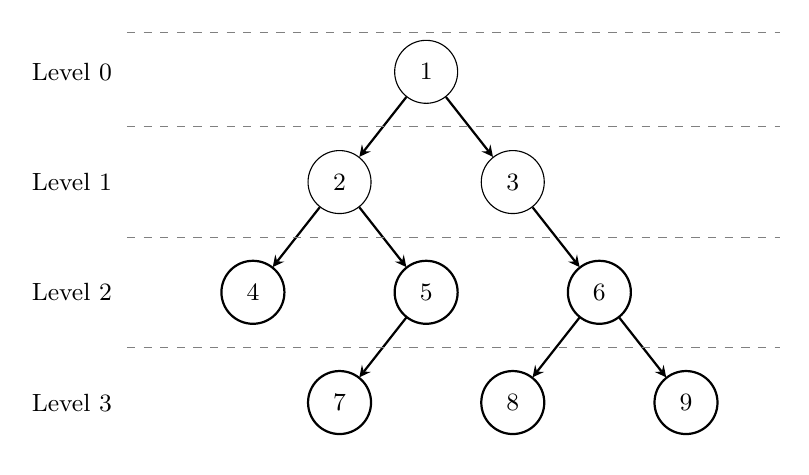
\begin{tikzpicture}[
  every node/.style={circle, draw, minimum size=0.8cm, font=\small, inner sep=1pt},
  level distance=1.4cm,
  sibling distance=2.2cm,
  edge from parent/.style={draw, ->, >=stealth, thick}
]
\node {1}
  child { node {2}
    child { node {4} }
    child { node {5}
      child { node {7} }
      child[missing] {}
    }
  }
  child { node {3}
    child[missing] {}
    child { node {6}
      child { node {8} }
      child { node {9} }
    }
  };

\node[draw=none, minimum size=0pt] at (-4.5, 0) {Level 0};
\node[draw=none, minimum size=0pt] at (-4.5, -1.4) {Level 1};
\node[draw=none, minimum size=0pt] at (-4.5, -2.8) {Level 2};
\node[draw=none, minimum size=0pt] at (-4.5, -4.2) {Level 3};

\draw[dashed, gray] (-3.8, 0.5) -- (4.5, 0.5);
\draw[dashed, gray] (-3.8, -0.7) -- (4.5, -0.7);
\draw[dashed, gray] (-3.8, -2.1) -- (4.5, -2.1);
\draw[dashed, gray] (-3.8, -3.5) -- (4.5, -3.5);

\end{tikzpicture}
\caption{A binary tree with 9 nodes. The root (node 1) has depth 0 and height 3. Node 7, 8, 9, and 4 are leaf nodes at levels 3 and 2.}
\label{fig:binary_tree_example}
\end{figure}

\subsection{Binary Tree Node Representation}
We represent a binary tree node in Java as follows:

\begin{verbatim}
class Node {
    int data;
    Node left;
    Node right;

    Node(int data) {
        this.data = data;
        this.left = null;
        this.right = null;
    }
}
\end{verbatim}

Each \texttt{Node} object is allocated on the heap and contains three fields: an integer payload (\texttt{data}), and two reference pointers to its left and right children. When a child does not exist, the reference is \texttt{null}.

\section{Classification of Binary Trees}
\label{sec:types}

Binary trees are classified into three canonical forms based on their structural constraints:

\subsection{Full (Proper/Strict) Binary Tree}
\begin{definition}[Full Binary Tree]
A binary tree is \emph{full} (or \emph{proper} or \emph{strict}) if every internal node has exactly 2 children. Equivalently, no node has exactly one child.
\end{definition}

\subsection{Complete Binary Tree}
\begin{definition}[Complete Binary Tree]
A binary tree of height $h$ is \emph{complete} if all levels $0, 1, \ldots, h-1$ are completely filled, and the last level $h$ is filled from left to right without gaps.
\end{definition}

Complete binary trees are the basis for the \emph{binary heap} data structure and can be efficiently stored in an array using index arithmetic: for a node at index $i$ (0-based), its left child is at $2i + 1$ and right child at $2i + 2$.

\subsection{Perfect Binary Tree}
\begin{definition}[Perfect Binary Tree]
A binary tree of height $h$ is \emph{perfect} if all internal nodes have exactly 2 children and all leaf nodes are at the same level $h$.
\end{definition}

\begin{theorem}[Node Count in a Perfect Binary Tree]
A perfect binary tree of height $h$ has exactly $2^{h+1} - 1$ total nodes.
\end{theorem}
\begin{proof}
At level $k$ ($0 \le k \le h$), there are exactly $2^k$ nodes. The total number of nodes is:
\begin{align}
    N &= \sum_{k=0}^{h} 2^k = 2^{h+1} - 1
\end{align}
This follows directly from the geometric series sum formula $\sum_{k=0}^{n} r^k = \frac{r^{n+1} - 1}{r - 1}$ with $r = 2$.
\end{proof}

\begin{corollary}
The number of leaf nodes in a perfect binary tree of height $h$ is $2^h$, which equals the number of internal nodes plus one.
\end{corollary}

\begin{figure}[htbp]
\centering
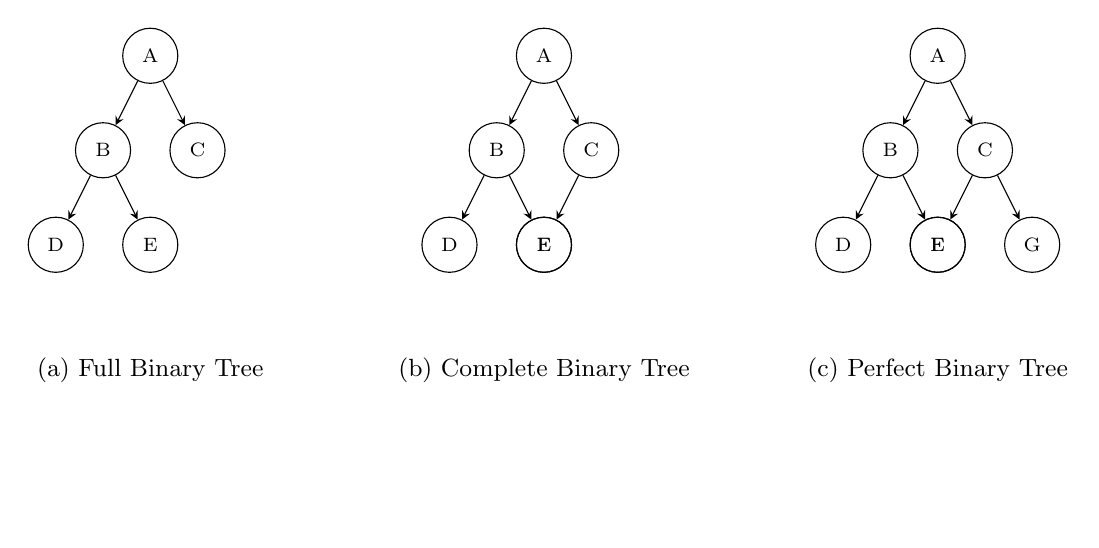
\begin{tikzpicture}[
  every node/.style={circle, draw, minimum size=0.7cm, font=\scriptsize, inner sep=1pt},
  level distance=1.2cm,
  sibling distance=1.2cm,
  edge from parent/.style={draw, ->, >=stealth}
]
% Full Binary Tree
\begin{scope}[xshift=-5cm]
\node {A}
  child { node {B}
    child { node {D} }
    child { node {E} }
  }
  child { node {C} };
\node[draw=none, minimum size=0pt, font=\small] at (0, -4) {(a) Full Binary Tree};
\end{scope}

% Complete Binary Tree
\begin{scope}[xshift=0cm]
\node {A}
  child { node {B}
    child { node {D} }
    child { node {E} }
  }
  child { node {C}
    child { node {F} }
    child[missing] {}
  };
\node[draw=none, minimum size=0pt, font=\small] at (0, -4) {(b) Complete Binary Tree};
\end{scope}

% Perfect Binary Tree
\begin{scope}[xshift=5cm]
\node {A}
  child { node {B}
    child { node {D} }
    child { node {E} }
  }
  child { node {C}
    child { node {F} }
    child { node {G} }
  };
\node[draw=none, minimum size=0pt, font=\small] at (0, -4) {(c) Perfect Binary Tree};
\end{scope}

\end{tikzpicture}
\caption{Classification of binary trees. (a) Full: every node has 0 or 2 children. (b) Complete: all levels filled except possibly the last, which is filled left-to-right. (c) Perfect: all internal nodes have 2 children and all leaves are at the same level.}
\label{fig:tree_types}
\end{figure}

Table~\ref{tab:tree_bounds} summarizes the node count bounds for each classification.

\begin{table}[htbp]
\centering
\caption{Node Count Bounds for Binary Tree Classifications (height $h$).}
\label{tab:tree_bounds}
\begin{tabular}{lccc}
\toprule
Property & Full & Complete & Perfect \\
\midrule
Min Nodes & $2h + 1$ & $2^h$ & $2^{h+1} - 1$ \\
Max Nodes & $2^{h+1} - 1$ & $2^{h+1} - 1$ & $2^{h+1} - 1$ \\
Leaves at level $h$ & $\ge 1$ & $\ge 1$ & $2^h$ \\
Array Representation & No & Yes & Yes \\
\bottomrule
\end{tabular}
\end{table}

\section{Recursive Depth-First Traversal Strategies}
\label{sec:recursive_traversals}

Tree traversal is the process of visiting every node in the tree exactly once in a defined order. The three canonical \emph{depth-first} traversal strategies are defined by the position at which the root is processed relative to its subtrees.

\subsection{Pre-order Traversal (Root $\to$ Left $\to$ Right)}

In pre-order traversal, we first process the current node, then recursively traverse the left subtree, and finally recursively traverse the right subtree.

\begin{verbatim}
void preorder(Node root) {
    if (root == null) {
        return;  // Base case: empty subtree
    }
    System.out.print(root.data + " ");  // Process root
    preorder(root.left);                 // Recurse left
    preorder(root.right);                // Recurse right
}
\end{verbatim}

\textbf{Pre-order applications:} Creating a copy of the tree, serializing tree structure for reconstruction, and generating prefix expressions from expression trees.

\subsection{In-order Traversal (Left $\to$ Root $\to$ Right)}

In in-order traversal, we first recursively traverse the left subtree, then process the current node, and finally recursively traverse the right subtree.

\begin{verbatim}
void inorder(Node root) {
    if (root == null) {
        return;  // Base case: empty subtree
    }
    inorder(root.left);                  // Recurse left
    System.out.print(root.data + " ");  // Process root
    inorder(root.right);                 // Recurse right
}
\end{verbatim}

\textbf{In-order applications:} For Binary Search Trees (BSTs), in-order traversal produces elements in sorted (non-decreasing) order, making it useful for validation and sorted output.

\subsection{Post-order Traversal (Left $\to$ Right $\to$ Root)}

In post-order traversal, we first recursively traverse the left subtree, then recursively traverse the right subtree, and finally process the current node.

\begin{verbatim}
void postorder(Node root) {
    if (root == null) {
        return;  // Base case: empty subtree
    }
    postorder(root.left);                // Recurse left
    postorder(root.right);               // Recurse right
    System.out.print(root.data + " ");  // Process root
}
\end{verbatim}

\textbf{Post-order applications:} Deleting a tree (children must be freed before their parent), evaluating postfix expressions, and computing directory sizes in file systems.

\subsection{Execution Trace (Dry Run)}

Consider the binary tree from Figure~\ref{fig:binary_tree_example} with nodes $\{1, 2, 3, 4, 5, 6, 7, 8, 9\}$. We trace each traversal order:

\begin{table}[htbp]
\centering
\caption{Traversal Output for the Binary Tree in Figure~\ref{fig:binary_tree_example}.}
\label{tab:traversal_output}
\begin{tabular}{ll}
\toprule
Traversal Strategy & Output Sequence \\
\midrule
Pre-order (Root-Left-Right) & $1, 2, 4, 5, 7, 3, 6, 8, 9$ \\
In-order (Left-Root-Right) & $4, 2, 7, 5, 1, 3, 8, 6, 9$ \\
Post-order (Left-Right-Root) & $4, 7, 5, 2, 8, 9, 6, 3, 1$ \\
\bottomrule
\end{tabular}
\end{table}

\subsection{Complexity Analysis}
\begin{theorem}
All three recursive depth-first traversals run in $O(N)$ time and $O(H)$ auxiliary space, where $N$ is the number of nodes and $H$ is the height of the tree.
\end{theorem}
\begin{proof}
Each node is visited exactly once across all recursive calls, giving $O(N)$ total work. The space complexity is determined by the maximum depth of the recursion call stack. In the worst case (a skewed tree where $H = N - 1$), the space complexity is $O(N)$. In the best case (a balanced tree where $H = \lfloor \log_2 N \rfloor$), the space complexity is $O(\log N)$.
\end{proof}

\section{Level-Order Traversal (Breadth-First Search)}
\label{sec:level_order}

Unlike depth-first strategies that dive deep into subtrees, \emph{level-order traversal} (also known as Breadth-First Search, BFS) visits all nodes at depth $k$ before visiting any node at depth $k+1$. This is achieved using a FIFO queue.

\subsection{Algorithm}
\begin{enumerate}
    \item Initialize a queue $Q$ and enqueue the root node.
    \item While $Q$ is not empty:
    \begin{enumerate}
        \item Dequeue a node $c$ from the front of $Q$.
        \item Process (print) $c$.
        \item If $c.\texttt{left} \neq \texttt{null}$, enqueue $c.\texttt{left}$.
        \item If $c.\texttt{right} \neq \texttt{null}$, enqueue $c.\texttt{right}$.
    \end{enumerate}
\end{enumerate}

\subsection{Java Implementation}
\begin{verbatim}
import java.util.Queue;
import java.util.LinkedList;

void levelOrder(Node root) {
    if (root == null) return;

    Queue<Node> q = new LinkedList<>();
    q.add(root);

    while (!q.isEmpty()) {
        Node curr = q.remove();
        System.out.print(curr.data + " ");

        if (curr.left != null) {
            q.add(curr.left);
        }
        if (curr.right != null) {
            q.add(curr.right);
        }
    }
}
\end{verbatim}

\subsection{Execution Trace}
For the tree in Figure~\ref{fig:binary_tree_example}, the level-order traversal proceeds as follows:

\begin{table}[htbp]
\centering
\caption{Level-Order BFS Execution Trace.}
\label{tab:bfs_trace}
\begin{tabular}{clll}
\toprule
Step & Dequeued Node & Queue State After & Output So Far \\
\midrule
1 & 1 & $\langle 2, 3 \rangle$ & 1 \\
2 & 2 & $\langle 3, 4, 5 \rangle$ & 1, 2 \\
3 & 3 & $\langle 4, 5, 6 \rangle$ & 1, 2, 3 \\
4 & 4 & $\langle 5, 6 \rangle$ & 1, 2, 3, 4 \\
5 & 5 & $\langle 6, 7 \rangle$ & 1, 2, 3, 4, 5 \\
6 & 6 & $\langle 7, 8, 9 \rangle$ & 1, 2, 3, 4, 5, 6 \\
7 & 7 & $\langle 8, 9 \rangle$ & 1, 2, 3, 4, 5, 6, 7 \\
8 & 8 & $\langle 9 \rangle$ & 1, 2, 3, 4, 5, 6, 7, 8 \\
9 & 9 & $\langle \rangle$ & 1, 2, 3, 4, 5, 6, 7, 8, 9 \\
\bottomrule
\end{tabular}
\end{table}

\begin{figure}[htbp]
\centering
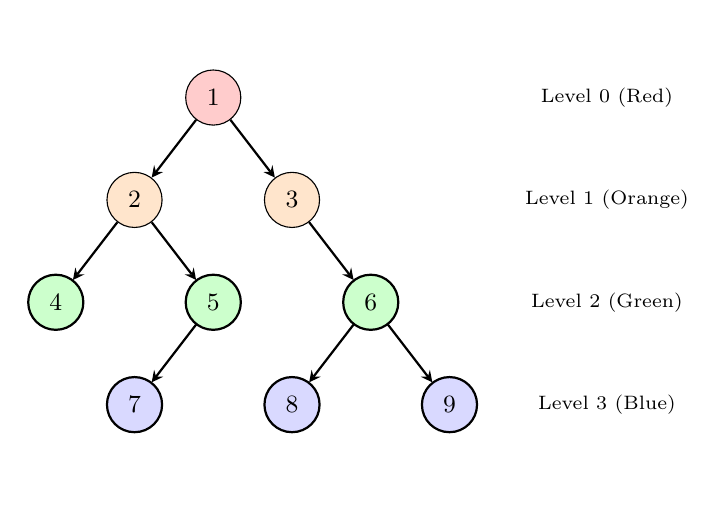
\begin{tikzpicture}[
  every node/.style={circle, draw, minimum size=0.7cm, font=\small, inner sep=1pt},
  level distance=1.3cm,
  sibling distance=2.0cm,
  edge from parent/.style={draw, ->, >=stealth, thick}
]
\node[fill=red!20] {1}
  child { node[fill=orange!20] {2}
    child { node[fill=green!20] {4} }
    child { node[fill=green!20] {5}
      child { node[fill=blue!15] {7} }
      child[missing] {}
    }
  }
  child { node[fill=orange!20] {3}
    child[missing] {}
    child { node[fill=green!20] {6}
      child { node[fill=blue!15] {8} }
      child { node[fill=blue!15] {9} }
    }
  };

\node[draw=none, minimum size=0pt, font=\scriptsize] at (5.0, 0) {Level 0 (Red)};
\node[draw=none, minimum size=0pt, font=\scriptsize] at (5.0, -1.3) {Level 1 (Orange)};
\node[draw=none, minimum size=0pt, font=\scriptsize] at (5.0, -2.6) {Level 2 (Green)};
\node[draw=none, minimum size=0pt, font=\scriptsize] at (5.0, -3.9) {Level 3 (Blue)};

\end{tikzpicture}
\caption{Level-order (BFS) traversal visits nodes level-by-level. Colors indicate the order: Level 0 (root) is processed first, then Level 1, then Level 2, and finally Level 3.}
\label{fig:level_order}
\end{figure}

\subsection{Complexity Analysis}
\begin{theorem}
Level-order traversal runs in $O(N)$ time and $O(W)$ auxiliary space, where $W$ is the maximum width (maximum number of nodes at any single level) of the tree.
\end{theorem}
\begin{proof}
Each of the $N$ nodes is enqueued and dequeued exactly once, each operation taking $O(1)$ time. Thus the total time is $O(N)$. The queue holds at most $W$ nodes simultaneously, where $W$ is the width of the widest level. For a perfect binary tree of height $h$, $W = 2^h = \frac{N+1}{2} = O(N)$ in the worst case. For a skewed tree, $W = 1$, giving $O(1)$ space.
\end{proof}

\section{Binary Tree View Projections}
\label{sec:views}

View projections extract the visible nodes when a binary tree is observed from a particular direction. These are computed using modified level-order traversals.

\subsection{Left View}

The \emph{Left View} of a binary tree consists of the first node visible at each level when the tree is viewed from the left side. Formally, it is the set of nodes $\{v_k : v_k \text{ is the first node at level } k\}$ for $k = 0, 1, \ldots, h$.

\subsubsection{Algorithm}
We perform a level-order traversal and, for each level, record only the \emph{first} node encountered:

\begin{verbatim}
import java.util.Queue;
import java.util.LinkedList;
import java.util.ArrayList;
import java.util.List;

List<Integer> leftView(Node root) {
    List<Integer> result = new ArrayList<>();
    if (root == null) return result;

    Queue<Node> q = new LinkedList<>();
    q.add(root);

    while (!q.isEmpty()) {
        int levelSize = q.size();

        for (int i = 0; i < levelSize; i++) {
            Node curr = q.remove();

            // First node of this level is the left view node
            if (i == 0) {
                result.add(curr.data);
            }

            if (curr.left != null) q.add(curr.left);
            if (curr.right != null) q.add(curr.right);
        }
    }
    return result;
}
\end{verbatim}

\subsection{Right View}

The \emph{Right View} of a binary tree consists of the last node visible at each level when the tree is viewed from the right side. Formally, it is the set of nodes $\{v_k : v_k \text{ is the last node at level } k\}$ for $k = 0, 1, \ldots, h$.

\subsubsection{Algorithm}
We perform the same level-order traversal but record the \emph{last} node at each level:

\begin{verbatim}
List<Integer> rightView(Node root) {
    List<Integer> result = new ArrayList<>();
    if (root == null) return result;

    Queue<Node> q = new LinkedList<>();
    q.add(root);

    while (!q.isEmpty()) {
        int levelSize = q.size();

        for (int i = 0; i < levelSize; i++) {
            Node curr = q.remove();

            // Last node of this level is the right view node
            if (i == levelSize - 1) {
                result.add(curr.data);
            }

            if (curr.left != null) q.add(curr.left);
            if (curr.right != null) q.add(curr.right);
        }
    }
    return result;
}
\end{verbatim}

\subsection{View Projection Trace}
For the binary tree in Figure~\ref{fig:binary_tree_example}:

\begin{table}[htbp]
\centering
\caption{Left View and Right View Projections.}
\label{tab:view_projections}
\begin{tabular}{clcc}
\toprule
Level & Nodes at Level & Left View & Right View \\
\midrule
0 & $\{1\}$ & 1 & 1 \\
1 & $\{2, 3\}$ & 2 & 3 \\
2 & $\{4, 5, 6\}$ & 4 & 6 \\
3 & $\{7, 8, 9\}$ & 7 & 9 \\
\bottomrule
\end{tabular}
\end{table}

\begin{figure}[htbp]
\centering
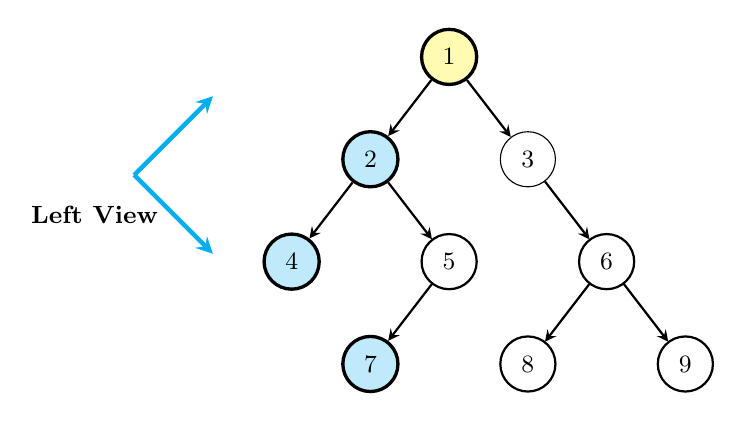
\begin{tikzpicture}[
  every node/.style={circle, draw, minimum size=0.7cm, font=\small, inner sep=1pt},
  level distance=1.3cm,
  sibling distance=2.0cm,
  edge from parent/.style={draw, ->, >=stealth, thick}
]
\node[fill=yellow!30, very thick] {1}
  child { node[fill=cyan!25, very thick] {2}
    child { node[fill=cyan!25, very thick] {4} }
    child { node {5}
      child { node[fill=cyan!25, very thick] {7} }
      child[missing] {}
    }
  }
  child { node {3}
    child[missing] {}
    child { node {6}
      child { node {8} }
      child { node {9} }
    }
  };

\node[draw=none, minimum size=0pt, font=\small] at (-4.5, -2) {\textbf{Left View}};
\draw[->, >=stealth, cyan, ultra thick] (-4.0, -1.5) -- (-3.0, -0.5);
\draw[->, >=stealth, cyan, ultra thick] (-4.0, -1.5) -- (-3.0, -2.5);

\end{tikzpicture}
\hspace{1.5cm}
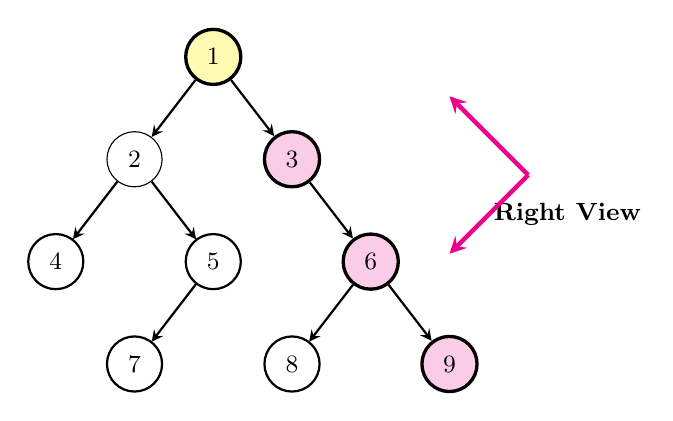
\begin{tikzpicture}[
  every node/.style={circle, draw, minimum size=0.7cm, font=\small, inner sep=1pt},
  level distance=1.3cm,
  sibling distance=2.0cm,
  edge from parent/.style={draw, ->, >=stealth, thick}
]
\node[fill=yellow!30, very thick] {1}
  child { node {2}
    child { node {4} }
    child { node {5}
      child { node {7} }
      child[missing] {}
    }
  }
  child { node[fill=magenta!20, very thick] {3}
    child[missing] {}
    child { node[fill=magenta!20, very thick] {6}
      child { node {8} }
      child { node[fill=magenta!20, very thick] {9} }
    }
  };

\node[draw=none, minimum size=0pt, font=\small] at (4.5, -2) {\textbf{Right View}};
\draw[->, >=stealth, magenta, ultra thick] (4.0, -1.5) -- (3.0, -0.5);
\draw[->, >=stealth, magenta, ultra thick] (4.0, -1.5) -- (3.0, -2.5);

\end{tikzpicture}
\caption{Left View (cyan highlighted nodes: 1, 2, 4, 7) and Right View (magenta highlighted nodes: 1, 3, 6, 9) of the binary tree.}
\label{fig:views}
\end{figure}

\subsection{Complexity Analysis}
\begin{theorem}
Both Left View and Right View algorithms run in $O(N)$ time and $O(W)$ auxiliary space.
\end{theorem}
\begin{proof}
The algorithms perform a standard level-order traversal, visiting each of the $N$ nodes exactly once. The conditional check ($i == 0$ for Left View, $i == \texttt{levelSize} - 1$ for Right View) adds only $O(1)$ overhead per node. The queue stores at most $W$ nodes at any time, where $W$ is the maximum tree width. Therefore, the time complexity is $O(N)$ and the space complexity is $O(W)$.
\end{proof}

\section{Summary of Complexity Bounds}

Table~\ref{tab:complexity_summary} consolidates the time and space complexities of all algorithms presented in this paper.

\begin{table}[htbp]
\centering
\caption{Consolidated Complexity Analysis of Binary Tree Algorithms.}
\label{tab:complexity_summary}
\begin{tabular}{lccc}
\toprule
Algorithm & Time & Aux. Space (Balanced) & Aux. Space (Skewed) \\
\midrule
Pre-order Traversal & $O(N)$ & $O(\log N)$ & $O(N)$ \\
In-order Traversal & $O(N)$ & $O(\log N)$ & $O(N)$ \\
Post-order Traversal & $O(N)$ & $O(\log N)$ & $O(N)$ \\
Level-order (BFS) & $O(N)$ & $O(N/2) = O(N)$ & $O(1)$ \\
Left View & $O(N)$ & $O(N)$ & $O(1)$ \\
Right View & $O(N)$ & $O(N)$ & $O(1)$ \\
\bottomrule
\end{tabular}
\end{table}

\section{Conclusion}
This paper has presented a formal algorithmic treatment of binary tree data structures. We established precise definitions for core tree terminology, classified binary trees into Full, Complete, and Perfect forms, and derived the node count bound $2^{h+1} - 1$ for perfect trees using geometric series. We formalized the three recursive depth-first traversal strategies (Pre-order, In-order, Post-order), providing complete Java implementations with dry-run execution traces. We introduced level-order (BFS) traversal as an iterative approach using a FIFO queue, proving its $O(N)$ time and $O(W)$ space bounds. Finally, we presented Left View and Right View algorithms as specialized level-order traversals that project the first and last visible nodes at each depth level respectively. The interplay between recursive depth-first and iterative breadth-first approaches highlights the fundamental trade-offs in tree algorithm design: recursion leverages the call stack for implicit state management at the cost of $O(H)$ stack space, while iteration with explicit queues provides $O(W)$ space behavior that adapts to tree shape.

\end{document}
